% ============================================================================
%  Institutional Representation ABM — JASSS draft
%
%  This is a FIRST-PASS DRAFT intended as a scaffold for human editing.
%
%  - Sections 1 (Introduction) and 6 (Discussion) are my best-guess framings
%    based on the Phase A–G analyses and the cited literature. They need
%    political-science-discipline review before submission; in particular,
%    the mechanism-as-aggregation framing (§6.2) is one of several defensible
%    readings and may not survive contact with a domain reviewer.
%  - Sections 3–5 are extracted mechanically from the phase notes and should
%    be more stable.
%  - The plausibility paragraph in §2 uses real benchmarks (see §11) but the
%    prose wrapping them is also a best guess.
%
%  Build:   cd paper && make
%  Requires pdflatex + bibtex. Figures are under ../docs/figures/.
% ============================================================================

\documentclass[11pt]{article}

\usepackage[margin=1in]{geometry}
\usepackage{graphicx}
\usepackage{booktabs}
\usepackage{amsmath}
\usepackage{amssymb}
\usepackage{siunitx}
\usepackage{url}
\usepackage[numbers,sort&compress]{natbib}
\usepackage{hyperref}
\hypersetup{
    colorlinks=true,
    linkcolor=black,
    citecolor=blue!60!black,
    urlcolor=blue!60!black,
}
\usepackage{caption}
\captionsetup{font=small, labelfont=bf}
\usepackage{microtype}
\usepackage{xcolor}

% Compact section headers
\usepackage{titlesec}
\titleformat*{\section}{\large\bfseries}
\titleformat*{\subsection}{\normalsize\bfseries}

% Allow \texttt{} to break at underscores in long identifiers. This eliminates
% most overfull hboxes without resorting to a global \sloppy.
\usepackage[htt]{hyphenat}

\graphicspath{{../docs/figures/}}

\title{%
    Why parliamentary systems collapse under fragmentation: \\
    A four-institution agent-based model of legislative passage
}
\author{%
    Fuad Ali
}
\date{\today}

\begin{document}
\maketitle

% ----------------------------------------------------------------------------
\begin{abstract}
\noindent
Parliamentary systems pass more bills than presidential systems at baseline,
but collapse to near-zero passage under party-system fragmentation. Three
competing micro-explanations --- coalition-formation failure, party
discipline, and committee gatekeeping --- are difficult to separate in
observational data because they operate simultaneously in any real
legislature. We present an agent-based model that compares four democratic
institutions: pure parliamentary, pure republican/presidential,
premier-presidential (France), and president-parliamentary (Russia). The
two semi-presidential variants are reachable from a single model class
through configurable toggles on government formation and presidential
dismissal power. Across four scenarios (baseline, fragmented, polarised,
small-system) and $N=200$ seeds per cell we report bootstrap confidence
intervals, Morris screening, Sobol variance decomposition, and mechanism
ablations. Two findings emerge. First, party discipline is the mechanism
majority-dependent institutions use to aggregate votes; disabling it
restores parliamentary passage from $0.05\%$ to $46.7\%$ under fragmentation,
and the rescue magnitude is monotone across the four institutions in a
pattern that survives varying the common discipline level. Second, the
passage--representation tradeoff is a single spectrum: parliamentary
maximises legislative throughput at the cost of representational fidelity;
republican maximises fidelity via the presidential veto at the cost of
throughput; semi-presidential variants split the difference. Together
these reframe the fragmentation-collapse literature: the collapse is a
discipline problem amplified by majority-rule government formation, not a
coalition-formation pathology on its own.

\medskip
\noindent\textbf{Keywords:} legislative studies, institutional design,
party discipline, coalition formation, semi-presidentialism, agent-based
modelling, Morris screening, Sobol sensitivity.
\end{abstract}

% ============================================================================
\section{Introduction}
\label{sec:intro}

Democracies differ dramatically in how much legislation they produce. In the
United Kingdom, over $95\%$ of government bills reach Royal Assent and
government defeats on second reading have not occurred since 1986
\citep{HoCLibraryCBP10489}. Germany passes roughly $90\%$ of
government-initiated bills \citep{dalton2009}. In contrast, only $3$--$7\%$
of bills introduced to the U.S. Congress are enacted into law, though most of
that figure reflects filtering at committee stage rather than genuine floor
rejection \citep{govtrack2023}. France, a premier-presidential system, enacts
roughly $70\%$ of its laws through government-sponsored \emph{projets de loi}
\citep{frenchlegprocess}. Russia's State Duma, a president-parliamentary
system, passes essentially $100\%$ of presidential bills while opposition
initiatives succeed at below $1\%$ \citep{noble2017}.

These differences reflect institutional rules rather than underlying
preferences: the cross-national variation in legislative productivity is
much larger than the cross-national variation in what electorates want. But
the rules interact in ways that are difficult to disentangle. Three
mechanistic accounts compete to explain why some legislatures produce laws
efficiently and others grind to a halt. The first emphasises
\textbf{coalition formation}: where a single party cannot hold a working
majority, bargaining over portfolios and policy may fail to produce a
viable government, blocking any legislative action before it starts
\citep{strom1990, laver2014}. The second emphasises \textbf{party
discipline}: strong whipping aligns MPs with their leadership rather than
their personal or constituent preferences, enabling the government to pass
bills that a free vote would reject \citep{bowler1999, cox1993}. The third
emphasises \textbf{committee gatekeeping}: structural rules that allow
small numbers of legislators to kill bills before floor consideration
\citep{shepsle1978, tsebelis2002}. These accounts are not mutually
exclusive, but their relative contributions to any observed passage pattern
are difficult to estimate because all three operate simultaneously in
every real legislature.

This paper uses an agent-based model (ABM) to attribute passage outcomes to
specific mechanisms. An ABM can implement coalition formation, party
discipline, and committee gatekeeping in a single deterministic simulation
and disable them one at a time while holding everything else fixed. The
mechanism-level counterfactuals required for causal attribution are
straightforward in a simulation and impossible in observational data.
Prior ABM work in legislative studies has typically modelled a single
mechanism at a time: coalition formation \citep{laver2014},
electoral mandate structure \citep{fowler2007}, and spatial voting in
the \citet{downs1957} tradition. Our contribution is to integrate the
three competing mechanisms in one framework and compare their
contributions across institutions and scenarios, building on the stylised
pattern that presidential systems achieve lower legislative success rates
than prime-ministerial systems while remaining robust to coalition failure
\citep{shugart2016, saiegh2014}.

We compare four institutional types. Pure \textbf{parliamentary} systems
follow the Westminster-Continental European template: the cabinet is drawn
from the legislature and falls on failed confidence votes. Pure
\textbf{republican} (presidential) systems follow the U.S. template: the
executive is elected separately, has formal veto power, and is not
responsible to the legislature. Between these two sit the
\textbf{semi-presidential} variants classified by \citet{shugart1992}.
\textbf{Premier-presidential} systems (France, Portugal, Ireland) have a
directly elected president alongside a cabinet responsible to parliament,
but the cabinet is formed by parliamentary majority and the president cannot
unilaterally dismiss the prime minister. \textbf{President-parliamentary}
systems (Russia, Weimar Germany) have the same pair of offices but the
president forms the government and can dismiss the PM without a parliamentary
vote. In our model both variants are reachable from a single class through
two independent configuration toggles.

Across these four institutions we run $N=200$ random seeds per scenario,
report bootstrap $95\%$ confidence intervals, use Morris elementary-effects
screening and Sobol variance decomposition to identify the dominant
parameters, and run mechanism ablations (disabling committees, discipline,
or veto one at a time) to attribute passage contributions. We also check
the robustness of the main ordering by varying the common discipline level
applied to all institutions.

Two findings structure our contribution. First (\S\ref{sec:results}.4),
under fragmentation the \emph{no-discipline} ablation restores
parliamentary passage from $0.05\%$ to $46.7\%$, and the rescue magnitude
is monotone across the four institutions in the order
parliamentary $>$ premier-presidential $>$ president-parliamentary $>$
republican. Under polarisation the same monotone ordering holds in
magnitude but with the opposite sign: disabling discipline now costs
parliamentary $66$ percentage points of passage. The sign-flip reveals the
underlying mechanism: discipline is the tool majority-dependent
institutions use to aggregate votes, enabling passage when a cohesive
coalition can enforce its will and blocking passage when it cannot.
Second (\S\ref{sec:results}.5), the passage--representation tradeoff is a
single spectrum. Parliamentary passes the most bills but its passed-bill
ideology matches no particular filter (policy representation gap
$\approx +0.04$ at polarised). Republican filters aggressively through the
presidential veto (gap $\approx -0.53$ at polarised) at the cost of high
non-passage rates. Semi-presidential variants sit between.

The remainder of the paper proceeds as follows.
Section~\ref{sec:model} describes the model;
Section~\ref{sec:design} describes the experimental design;
Section~\ref{sec:results} presents the results;
Section~\ref{sec:discussion} discusses implications and relates the
findings to prior work; Section~\ref{sec:limitations} states limitations;
Section~\ref{sec:reproducibility} documents code, data, and the
interactive companion app.

% ============================================================================
\section{Model description}
\label{sec:model}

\subsection{Agents and state}
The model contains four agent types:
\textbf{constituencies} with a fixed two-dimensional ideology (economic
$\times$ social) and a population;
\textbf{parties} with an ideology and a name;
\textbf{legislators} with an ideology, an assigned constituency, and an
assigned party; and
\textbf{committees} with a policy-area jurisdiction (an ideology centre
and radius) and party-proportional membership.
Bills are ephemeral objects with an ideology and a salience, instantiated
per legislative step.

All four institutions share the same agent types and initialisation
procedure. They differ only in the bill-processing pipeline invoked by
\texttt{pass\_legislation(bill)} and in the institution-specific state that
pipeline reads and writes (government, cabinet, president, confidence votes,
vetoes, dismissals).

\subsection{Passage pipelines}
Parliamentary: bills route to a committee with matching jurisdiction
(committees can approve, amend, or kill); with probability
$\texttt{confidence\_matter\_rate}$ a bill is treated as a confidence vote
and whipped harder; a floor vote with party discipline decides passage;
failed confidence votes trigger government collapse and reformation.

Republican: bills route to a committee (with stronger gatekeeping power);
a floor vote with weak discipline decides legislative passage; the
executive vetoes probabilistically by ideological distance from the bill;
a two-thirds override attempt follows vetoes.

Semi-presidential: hybridises both pipelines. Committees route bills;
bills may be treated as confidence matters; a floor vote with moderate
discipline decides legislative passage; the directly-elected president
then checks a veto; if the president can dismiss the PM
(president-parliamentary variant) the dismissal check fires on every bill
and may collapse the government independently of confidence votes.

\subsection{Configuration toggles for semi-presidential variants}
Two \texttt{SemiPresidentialConfig} toggles distinguish the variants:

\begin{itemize}
    \item \texttt{government\_formation} $\in$ \{\texttt{majority\_driven},
        \texttt{president\_driven}\}. Majority-driven formation follows the
        parliamentary rule (largest party alone if it holds a majority,
        else two-party coalition). President-driven formation appoints the
        president's party as the governing party, adding a second party for
        majority only if available; otherwise a minority cabinet.
    \item \texttt{president\_can\_dismiss\_pm} $\in$ \{\texttt{False},
        \texttt{True}\}. When \texttt{True}, the president dismisses the PM
        with probability \texttt{presidential\_dismissal\_rate} whenever
        their ideological distance exceeds $0.5$.
\end{itemize}

Premier-presidential corresponds to
(\texttt{majority\_driven}, \texttt{False}); president-parliamentary to
(\texttt{president\_driven}, \texttt{True}). Non-canonical combinations are
reachable but not the focus here.

\subsection{ODD protocol}
A full ODD description \citep{grimm2010, grimm2020} appears in
Appendix~\ref{app:odd}. All agent states, scheduling, design concepts,
initialisation, and submodel equations are documented there.

% ============================================================================
\section{Experimental design}
\label{sec:design}

\subsection{Scenarios}
Four scenarios vary the political environment while holding institutional
rules fixed:
\textbf{baseline} ($20$ legislators, $3$ parties, $6$ constituencies, $25$
bills, bill ideology range $[-1, 1]$);
\textbf{fragmented} ($24$ legislators, $5$ parties, $8$ constituencies, $30$
bills, range $[-1, 1]$);
\textbf{polarised} ($16$ legislators, $2$ parties, $4$ constituencies, $20$
bills, range $[-1.5, 1.5]$); and
\textbf{small-system} ($10$ legislators, $2$ parties, $3$ constituencies,
$15$ bills, range $[-0.8, 0.8]$).

\subsection{Statistical harness}
Each (scenario, institution) cell is replicated over $N=200$ seeds. We
report means with percentile bootstrap $95\%$ confidence intervals
(\texttt{scipy.stats.bootstrap}, $9\,999$ resamples). Pairwise institution
comparisons use Welch's $t$-test and Mann-Whitney $U$; effect sizes are
reported as Cohen's $d$. When zero-variance cells produce undefined
$p$-values, those are recorded as \texttt{NaN} rather than imputed.

\subsection{Sensitivity analysis}
For each institution we define a six-parameter problem and run Morris
elementary-effects screening ($r=20$ trajectories, $4$ levels) and Sobol
variance decomposition ($N=256$ base samples, first-order and total-order
indices). Three seeds per design point reduce stochastic variance without
inflating cost. The six parameters per institution always include
\texttt{discipline\_strength}, \texttt{committee\_gatekeeping\_power},
\texttt{num\_parties}, and \texttt{num\_constituencies}; the remaining two
are institution-specific.

\subsection{Mechanism ablations}
Three ablations modify the running model without touching the production
code. \texttt{no\_committees} replaces the committee-routing function with
a pass-through; \texttt{no\_discipline} sets
\texttt{discipline\_strength = 0}; \texttt{no\_veto} (where applicable)
replaces the executive-veto check with \texttt{False}. Each ablation is
monkey-patched on the live model instance; no class-level mutation occurs.

\subsection{Discipline-default robustness check}
To test whether the observed ordering depends on our default
discipline values, we sweep a common discipline level
$D \in \{0.0, 0.1, \ldots, 0.9\}$ applied simultaneously to all four
institutions, and compute
$\mathrm{rescue}(D) = \mathrm{passage}(D=0) - \mathrm{passage}(D)$ per
institution at $N=100$ seeds per cell.

% ============================================================================
\section{Results}
\label{sec:results}

\subsection{Passage rates across scenarios}
\label{sec:results:passage}

Figure~\ref{fig:forest} summarises per-scenario mean passage rates with
$95\%$ bootstrap CIs for all four institutions. At baseline the expected
ordering holds: parliamentary $0.742$ [$0.729$, $0.754$], premier-presidential
$0.547$, president-parliamentary $0.546$, republican $0.450$
[$0.436$, $0.464$]. Parliamentary's advantage $(+29\text{pp})$ over republican
is highly significant (Welch's $t = 38.9$, $p < 10^{-200}$; Cohen's $d = 2.88$).

\begin{figure}[ht]
    \centering
    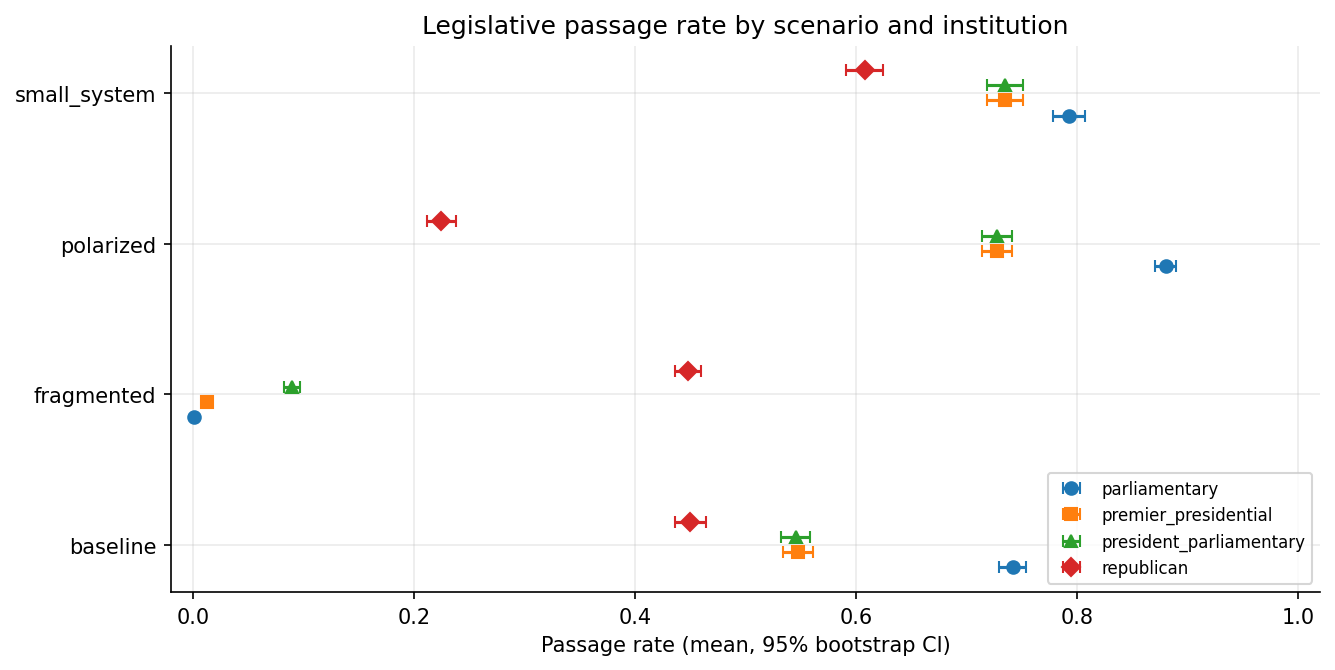
\includegraphics[width=0.85\linewidth]{forest_passage.png}
    \caption{Per-scenario mean passage rate with $95\%$ bootstrap CIs, for
    all four institutions ($N=200$ seeds per cell).}
    \label{fig:forest}
\end{figure}

\subsection{The fragmentation collapse}

Under fragmentation, parliamentary passage collapses to $0.001$
($0$--$0.001$ CI) while republican holds at $0.448$. The two
semi-presidential variants split: premier-presidential collapses to $0.013$
(similar to parliamentary because it shares the majority-driven formation
rule), while president-parliamentary partially rescues passage to $0.086$
through its president-driven minority-cabinet rule.
Figure~\ref{fig:violin} shows the per-seed distributions: the collapse is a
regime property, not a tail event.

\begin{figure}[ht]
    \centering
    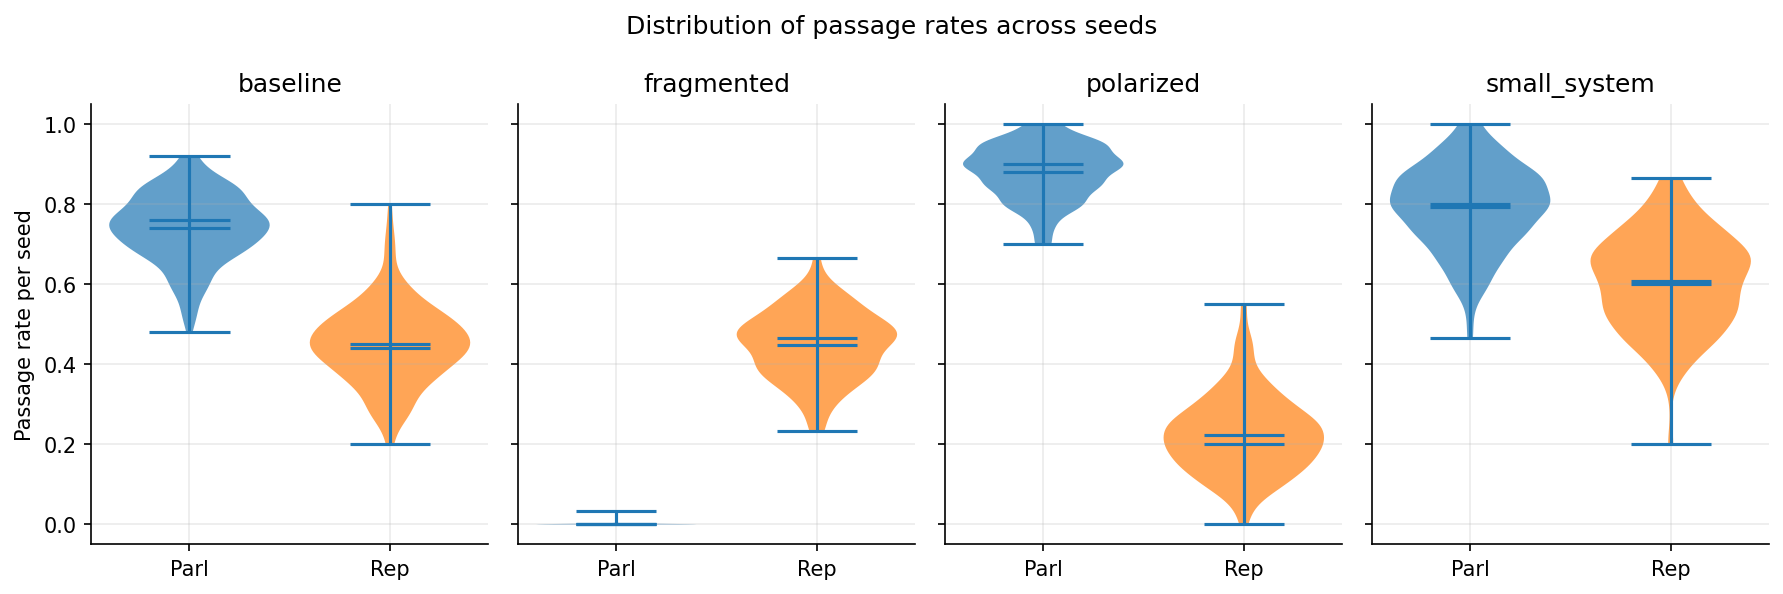
\includegraphics[width=0.95\linewidth]{violin_passage.png}
    \caption{Per-seed passage-rate distributions, faceted by scenario. The
    fragmented cell shows near-zero passage for both majority-driven
    institutions (parliamentary, premier-presidential) and a partial rescue
    under president-parliamentary.}
    \label{fig:violin}
\end{figure}

\subsection{Sensitivity: different institutions, different bottlenecks}

Sobol total-order indices at baseline (Fig.~\ref{fig:sobol}) show that
parliamentary passage is dominated by \texttt{num\_parties}
($S_T = 0.808$), consistent with the fragmentation-collapse finding.
Republican passage is dominated by
\texttt{committee\_gatekeeping\_power} ($S_T = 0.671$) with
\texttt{discipline\_strength} second ($S_T = 0.477$). The two institutions
have structurally different bottlenecks. Semi-presidential variants track
parliamentary in their dependence on \texttt{num\_parties}.

\begin{figure}[ht]
    \centering
    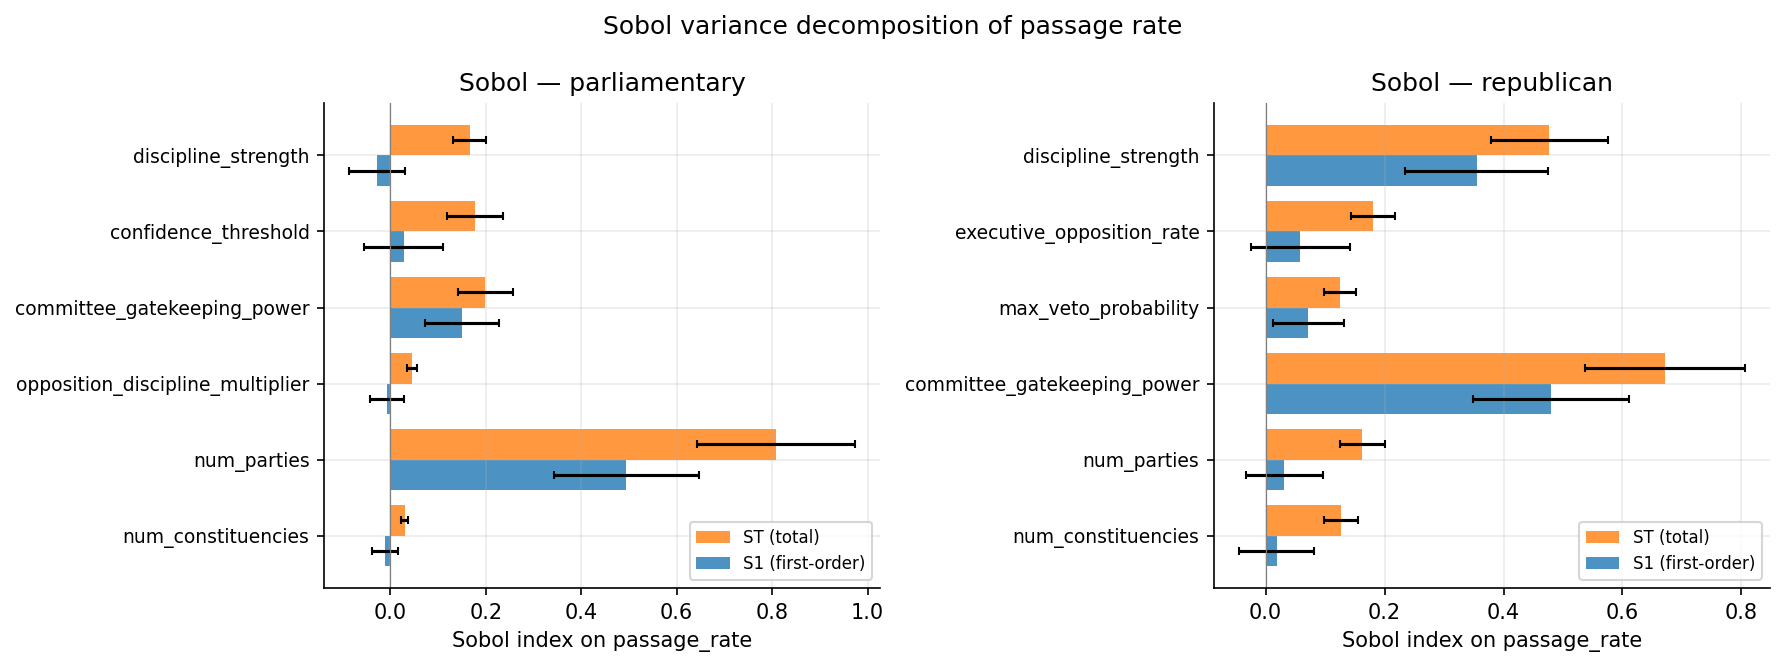
\includegraphics[width=0.95\linewidth]{sobol_bars.png}
    \caption{Sobol first-order ($S_1$) and total-order ($S_T$) indices for
    passage rate at baseline.}
    \label{fig:sobol}
\end{figure}

Running the same analysis on the fragmented scenario confirms the
num-parties dominance across all three majority-dependent institutions
($S_T \approx 0.76$--$0.79$) and reveals that
\texttt{confidence\_threshold} gains importance under fragmentation
($+0.12$ in $S_T$ for parliamentary). Republican remains structurally
insensitive to \texttt{num\_parties} ($S_T = 0.14$).

\subsection{Mechanism attribution via ablation}
\label{sec:results:ablation}

Figure~\ref{fig:ablation} shows $\Delta\text{passage\_rate}$ relative to
the full model for each (scenario, institution, ablation) cell at $N=200$.
The headline result appears at fragmented:

\begin{table}[ht]
    \centering
    \caption{\texttt{no\_discipline} ablation $\Delta$ under fragmentation.}
    \begin{tabular}{lcc}
        \toprule
        Institution & Full-model passage & $\Delta$ (no\_discipline $-$ full) \\
        \midrule
        parliamentary & $0.001$ & $+0.466$ \\
        premier\_presidential & $0.013$ & $+0.312$ \\
        president\_parliamentary & $0.086$ & $+0.233$ \\
        republican & $0.448$ & $-0.242$ \\
        \bottomrule
    \end{tabular}
    \label{tab:ablation-fragmented}
\end{table}

Disabling party discipline restores parliamentary passage from
near-zero to nearly $47\%$. The rescue magnitude decreases monotonically
across the four institutions in the order parliamentary $>$
premier-presidential $>$ president-parliamentary $>$ republican. Republican
is the only institution where zeroing discipline \emph{hurts} rather than
helps: without a majority-formation gate, discipline plays a different
role (crude vote aggregation on the floor) and removing it simply damages
the signal.

\begin{figure}[ht]
    \centering
    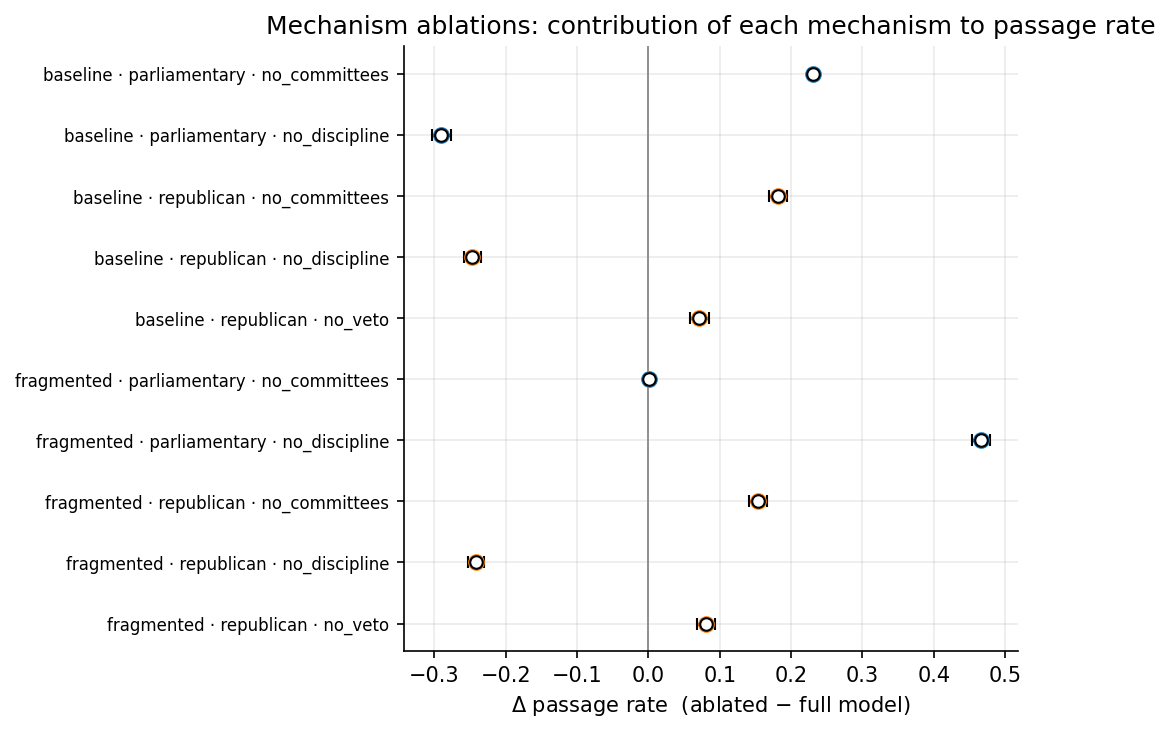
\includegraphics[width=0.85\linewidth]{ablation_forest.png}
    \caption{Ablation deltas ($\Delta$ passage rate relative to full model)
    for each (scenario, institution, ablation) cell at $N=200$ seeds.
    Confidence bars are $\pm 1.96\,\mathrm{SE}$.}
    \label{fig:ablation}
\end{figure}

Under polarised scenarios the same ordering holds in magnitude but with
opposite sign (Table~\ref{tab:ablation-polarized}). Discipline \emph{enables}
passage when the coalition wants extreme bills to pass; disabling
discipline costs parliamentary $66$ percentage points. Republican, with
no coalition to whip, loses only $11$ percentage points. The cross-scenario
pattern reveals that discipline is the mechanism majority-dependent
institutions use to \emph{aggregate votes}, not a mechanism that
specifically causes fragmentation pathologies.

\begin{table}[ht]
    \centering
    \caption{\texttt{no\_discipline} ablation $\Delta$ under polarisation.}
    \begin{tabular}{lcc}
        \toprule
        Institution & Full-model passage & $\Delta$ (no\_discipline $-$ full) \\
        \midrule
        parliamentary & $0.880$ & $-0.664$ \\
        premier\_presidential & $0.728$ & $-0.557$ \\
        president\_parliamentary & $0.723$ & $-0.557$ \\
        republican & $0.225$ & $-0.113$ \\
        \bottomrule
    \end{tabular}
    \label{tab:ablation-polarized}
\end{table}

\subsection{Passage--representation tradeoff}
\label{sec:results:tradeoff}

Figure~\ref{fig:tradeoff} plots passage rate against a new metric, the
policy representation gap:
\begin{equation}
    \mathrm{gap} \;=\; \overline{d_{\text{passed}}}
                     - \overline{d_{\text{proposed}}}
\end{equation}
where $d$ is the L2 distance between a bill's ideology and the
constituency-median ideology. Negative gaps indicate the institution
filters passed bills toward the median; positive gaps indicate the
institution spreads passed bills relative to random proposal draws.

\begin{figure}[ht]
    \centering
    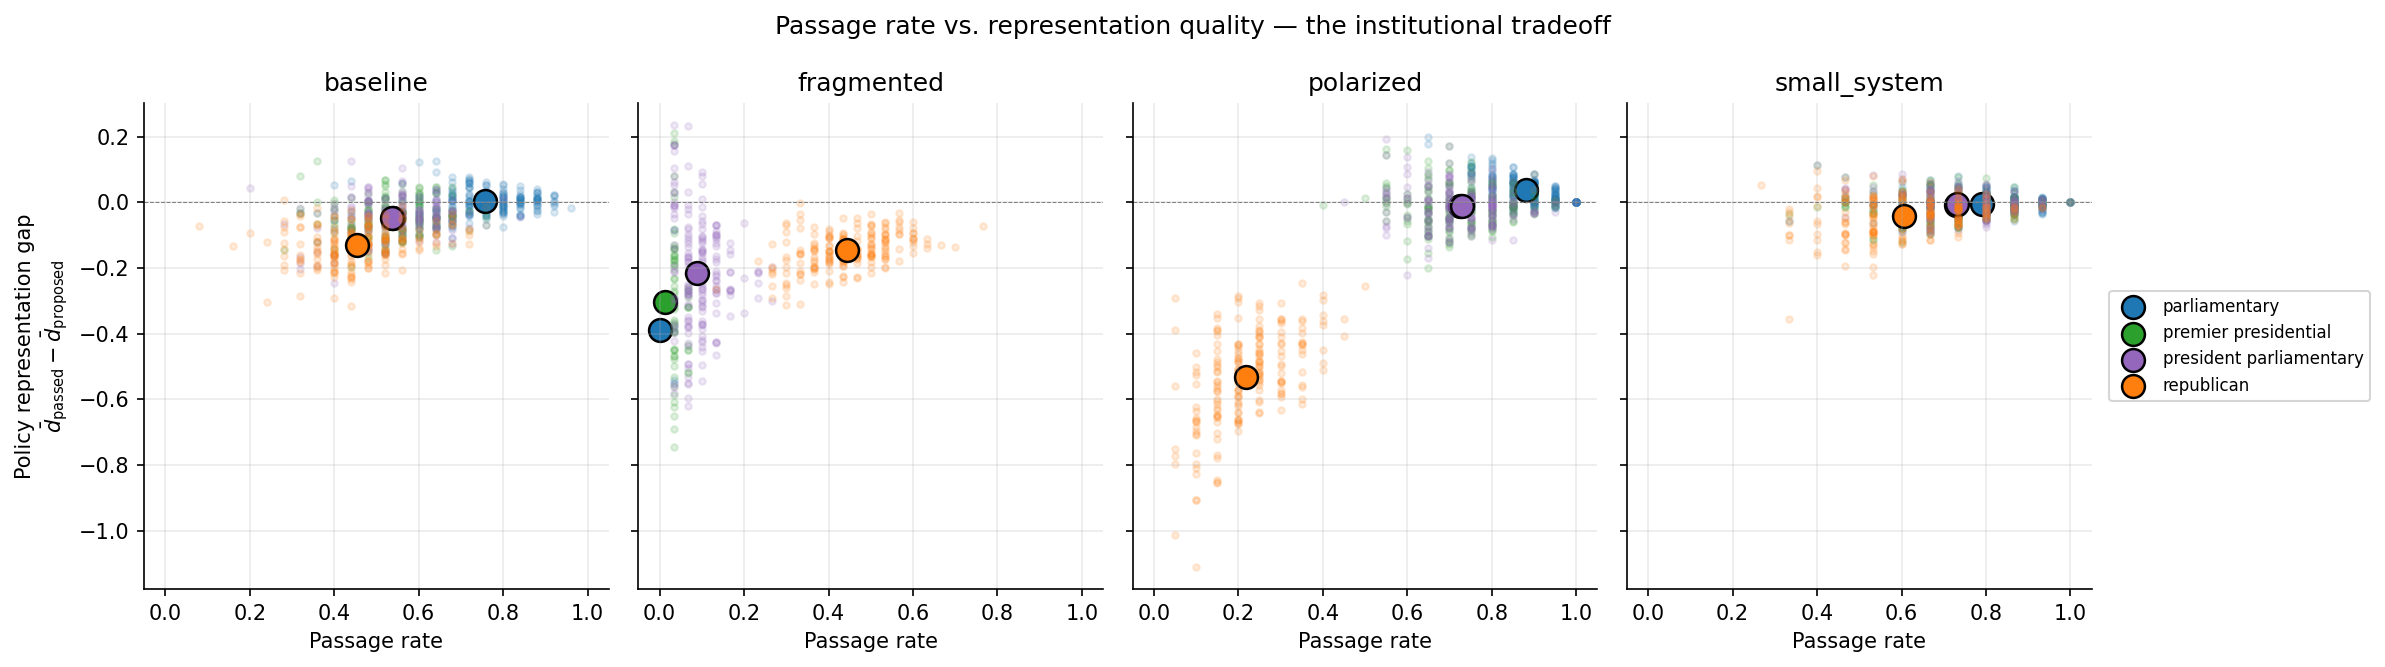
\includegraphics[width=0.98\linewidth]{representation_tradeoff.png}
    \caption{Passage rate versus policy representation gap, per scenario.
    Each large marker is the $N=200$ mean; the cloud is per-seed. Under
    polarisation the tradeoff is most visible: parliamentary at
    $(0.88, +0.04)$ vs.~republican at $(0.22, -0.53)$.}
    \label{fig:tradeoff}
\end{figure}

The tradeoff is sharpest under polarised scenarios:

\begin{table}[ht]
    \centering
    \caption{Passage--representation tradeoff at polarised ($N=200$).}
    \begin{tabular}{lcc}
        \toprule
        Institution & Passage rate & Representation gap \\
        \midrule
        parliamentary & $0.882$ & $+0.037$ \\
        premier\_presidential & $0.725$ & $-0.012$ \\
        president\_parliamentary & $0.730$ & $-0.010$ \\
        republican & $0.218$ & $-0.530$ \\
        \bottomrule
    \end{tabular}
    \label{tab:tradeoff-polarized}
\end{table}

Parliamentary passes $88\%$ of bills with essentially no ideological filter;
republican passes only $22\%$ but the bills that do pass are strongly
biased toward the constituent median, reflecting the presidential veto's
role as an ideological screen. Semi-presidential variants sit on the same
spectrum between them. Filtering and throughput are mechanistically
linked: any mechanism that increases one reduces the other.

\subsection{Robustness of the monotone ordering}

The ablation ordering in Table~\ref{tab:ablation-fragmented} could in
principle be an artefact of our default \texttt{discipline\_strength}
values, which happen to be ordered the same way across institutions
($0.8$, $0.6$, $0.6$, $0.4$). Figure~\ref{fig:robustness} tests this by
setting all four institutions' \texttt{discipline\_strength} to the same
value $D \in \{0.1, \ldots, 0.9\}$ and measuring the rescue magnitude.

\begin{figure}[ht]
    \centering
    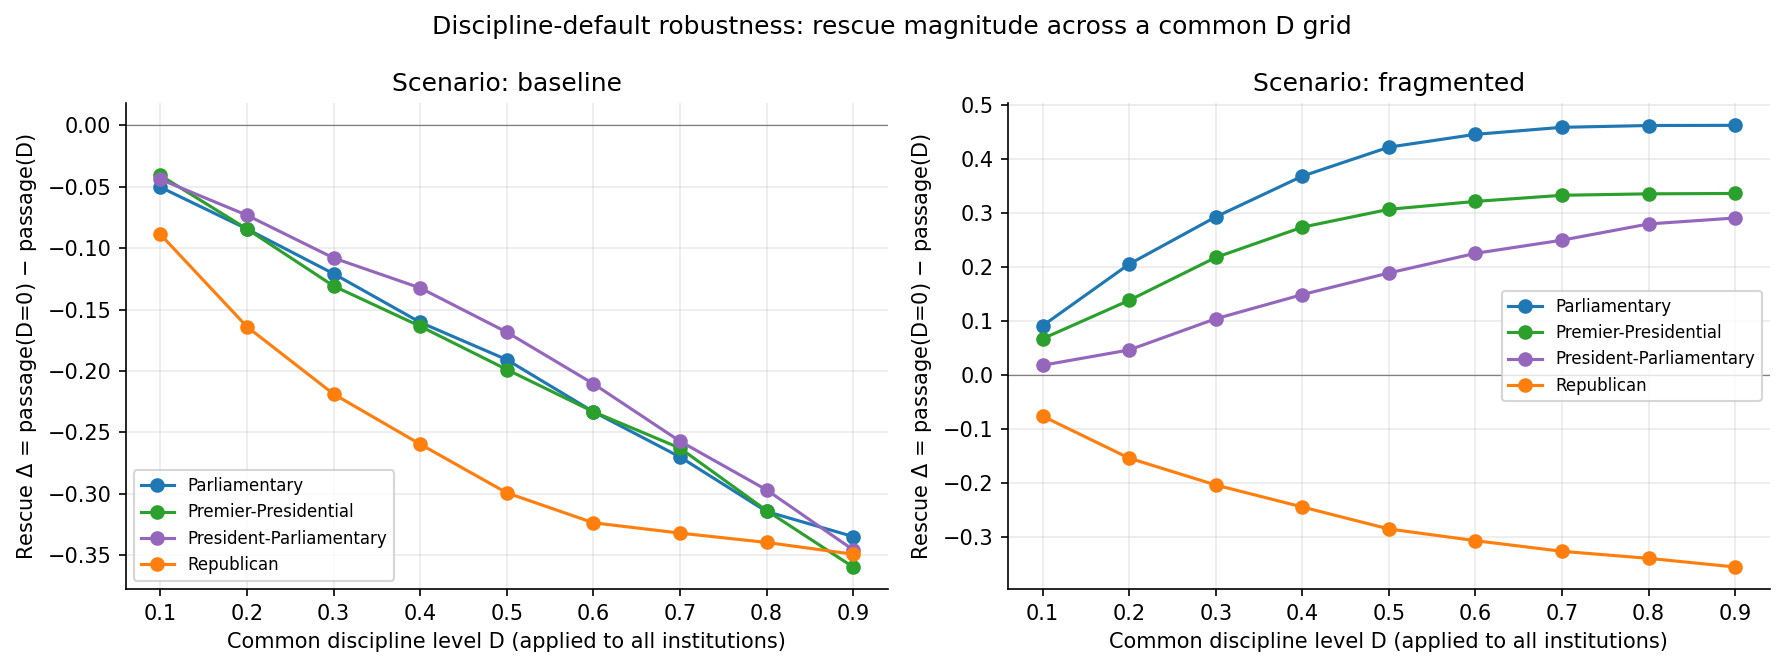
\includegraphics[width=0.98\linewidth]{discipline_rescue_curves.png}
    \caption{Rescue magnitude versus common discipline level $D$, per
    institution, at baseline and fragmented scenarios. Under fragmented
    (right panel), the monotone ordering parliamentary $>$
    premier-presidential $>$ president-parliamentary $>$ republican holds
    at all nine tested $D$ values.}
    \label{fig:robustness}
\end{figure}

The monotone ordering parliamentary $>$ premier-presidential $>$
president-parliamentary $>$ republican holds at $9/9$ tested $D$ values
under fragmentation. The structural claim survives: the ordering is not a
function of our chosen defaults. A regression test in the repository
enforces this at $D \in \{0.0, 0.2, 0.5, 0.8\}$ so that future mechanism
changes that break the ordering fail CI.

% ============================================================================
\section{Discussion}
\label{sec:discussion}

\subsection{Discipline as a universal aggregation mechanism}

The ablation results across fragmented and polarised scenarios
(Tables~\ref{tab:ablation-fragmented} and \ref{tab:ablation-polarized})
reveal that party discipline is not simply a ``collapse trigger''' under
fragmentation or a ``passage enabler'' under polarisation. It is the same
mechanism in both cases: discipline aggregates legislators toward the
coalition-leadership preference rather than the free-vote median. In
regimes where the coalition can form and its preferences are near the
floor median, discipline enforces passage. In regimes where the coalition
cannot form, discipline enforces an imaginary position that blocks passage.
The sign-flip between the two scenarios is a direct consequence of this
mechanism, not evidence of two separate mechanisms.

The monotone ordering across the four institutions reflects how much each
relies on a formation-gated coalition to act. Parliamentary requires a
majority coalition before any legislation is possible; premier-presidential
requires the same, but with a presidential veto adding a second gate;
president-parliamentary also nominally requires a majority, but the
president-driven formation rule lets the government function as a minority
cabinet when no majority forms; republican has no formation gate at all.
The rescue magnitude under \texttt{no\_discipline} scales with this
dependence. This reading is consistent with \citet{strom1990}'s argument
that minority governments can function when institutions permit, and with
\citet{shugart1992}'s typology of semi-presidential variants.

Crucially, this framing makes a prediction that a pure
``fragmentation-collapse'' framing does not: under polarisation, the same
institutions that suffered the fragmentation collapse should benefit most
from discipline. Table~\ref{tab:ablation-polarized} confirms this.

\subsection{The passage--representation tradeoff as a single spectrum}

Figure~\ref{fig:tradeoff} and Table~\ref{tab:tradeoff-polarized} make a
concrete claim about the tradeoff between legislative throughput and
representational fidelity: the two quantities lie on a single axis for the
four institutions studied. Parliamentary sits at one end (high throughput,
low filter); republican at the other (low throughput, high filter);
semi-presidential variants between them. The mechanism is
straightforward. Discipline-plus-majority passage, the parliamentary
mechanism, has no ideological test: whatever the coalition proposes
passes. The presidential veto, the republican mechanism, \emph{is} an
ideological test: bills far from the executive's ideology are filtered
probabilistically. Committees add filtering in both but the effect is
smaller than the presidential veto.

This casts the parliamentary ``advantage'' in baseline passage rates
differently. Parliamentary systems pass more bills in absolute terms but
do not necessarily pass \emph{better} bills in the sense of matching
constituent preferences. The comparison requires joint consideration of
both axes, not rank-ordering on one.

\subsection{Policy and institutional-design implications}

The conventional response to fragmented-parliament gridlock is
\emph{electoral reform}: raise thresholds, move toward first-past-the-post,
encourage larger parties. Our results suggest a second route:
\emph{discipline reform}. Allowing free votes on more bills, weakening
leadership whip powers, or restructuring MP incentives toward their
districts rather than their parties could in principle restore passage
capacity under fragmentation without touching electoral rules. Whether
such reforms also damage representation (the parliamentary filter is
already weak; weakening discipline further might spread passed bills
without the presidential-veto compensation) is an open empirical question
that this model can illuminate but not yet answer directly.

For new constitutional design, the Phase~F robustness result suggests a
trade-off between fragility and filtering. Pure parliamentary maximises
passage at baseline but has a failure mode under fragmentation;
president-parliamentary partially insulates against that failure mode but
sacrifices some passage at baseline; republican is robust at all
scenarios but pays a throughput tax. Premier-presidential is closer to
parliamentary than its name suggests and shares the fragmentation
vulnerability.

\subsection{Relation to prior work}

\citet{linz1990} argued parliamentary systems outperform presidential
systems in producing governments and policy. Our baseline results
($0.742$ vs.~$0.450$) echo that finding on passage rates, but our
fragmentation results reverse it: parliamentary collapses while presidential
holds steady. The conditional reversal recovers a pattern Linz's categorical
claim cannot predict. \citet{shugart1992} argued semi-presidential variants
should differ from each other in specific ways; we confirm that
president-parliamentary's partial rescue of passage under fragmentation is
a direct consequence of the president-driven formation rule. \citet{tsebelis2002}
argued additional veto players reduce policy mobility; our tradeoff finding
refines this by showing that veto players also improve representation
quality, so the choice is not ``veto players good or bad'' but ``veto
players trade throughput for filtering.''

% ============================================================================
\section{Limitations}
\label{sec:limitations}

The model treats legislator ideology as static and does not include
learning or adaptation. It has no endogenous party emergence, realignment,
or exit; the party structure is fixed at initialisation. It has no
bicameralism, judicial review, federalism, or presidential agenda-setting
powers beyond the veto. Bills have no path dependence: each bill is an
independent draw. We do not model pre-parliamentary agenda control (e.g.,
cabinet screening of government bills before introduction), which is why
our parliamentary baseline rate of $74\%$ is below the empirical UK and
German benchmarks of $90$--$95\%$ for government bills.

Cohabitation is detected in our semi-presidential runs (shares of
$12$--$26\%$ across scenarios) but does not produce meaningful passage
effects: our dismissal rate of $5\%$ per bill under president-parliamentary
is too gentle to create sustained gridlock, and the premier-presidential
presidential veto is too soft to differentially block bills under
cohabitation. A fuller treatment of cohabitation dynamics --- including
cabinet--legislator ideological alignment and differential veto thresholds
under divided government --- is deferred to future work.

The sensitivity analysis was run primarily on the baseline scenario; a
secondary run on the fragmented scenario (\S\ref{sec:results}.3) confirms
the \texttt{num\_parties} dominance but is not a substitute for per-scenario
sweeps of all parameters. The Morris and Sobol samplers include
\texttt{num\_parties} and \texttt{num\_constituencies} in the sweep space;
scenario definitions are therefore overlapping with the sensitivity space,
which is a methodological choice to allow continuous interpolation rather
than a discrete scenario lookup.

% ============================================================================
\section{Reproducibility}
\label{sec:reproducibility}

All results are deterministic under seed. The repository
\url{https://github.com/tofuadmiral/institutional-representation-abm} contains
the full code, $68$ automated tests (Python 3.13 on Ubuntu, GitHub Actions
CI), a pinned regression fixture, a Streamlit interactive companion
application, and a CoMSES metadata card. The command
\begin{verbatim}
python -m experiments.multiseed_comparison --scenarios all --seeds 200
\end{verbatim}
reproduces Figure~\ref{fig:forest}.
Tables~\ref{tab:ablation-fragmented} and \ref{tab:ablation-polarized}
require additional invocations of \texttt{experiments.ablation};
Figure~\ref{fig:robustness} requires
\texttt{experiments.discipline\_robustness}; and
Figure~\ref{fig:tradeoff} requires \texttt{experiments.representation}.
All entry points are documented in the repository \texttt{README.md}.
Full runtime is under five minutes on eight cores. An interactive
Streamlit companion (\texttt{streamlit run streamlit\_app/app.py})
exposes every tunable configuration parameter as a slider and reproduces
the scenario-comparison, parameter-sweep, and ablation workflows used in
\S\ref{sec:results}.

% ============================================================================
\appendix

\section{ODD Protocol}
\label{app:odd}

The full ODD protocol \citep{grimm2010, grimm2020} is available in the
repository at \texttt{docs/ODD\_PROTOCOL.md}. Core elements are summarised
in \S\ref{sec:model}.

% ============================================================================
\bibliographystyle{plainnat}
\bibliography{references}

\end{document}
